% Chapter Template

\chapter{Conclusion} % Main chapter title

\label{Chapter9} % Change X to a consecutive number; for referencing this chapter elsewhere, use \ref{ChapterX}

\lhead{Chapter 9. \emph{Conclusion}} % Change X to a consecutive number; this is for the header on each page - perhaps a shortened title

%----------------------------------------------------------------------------------------
%	SECTION 1
%----------------------------------------------------------------------------------------

\section{Summary}

In summary, this project aims to develop an application that can count sheets of cloth with the acceptable accuracy result. It is expected to reduce hospital staff’s fatigue in manual sheets counting. An input image should have enough contrast and there should be no pattern on the cloth. Furthermore, the sheets of cloth should be of the same color. Each layer the width of sheets of cloth should cover more than ten pixels. 

%----------------------------------------------------------------------------------------
%	SECTION 2
%----------------------------------------------------------------------------------------

\section{Lessons learned}
Throughout the semester, two of the most important lessons we all have learned are teamwork and communication skills. When we are teamwork the good communication skill is important.

Beside what is previous mention, we have learned lesson as follows:
\begin{itemize}
	\item {MATLAB programming}
	\item {iOS application development}
	\item {Image processing techniques}
	\item {Machine Learning (for data cluttering)}
\end{itemize}
%----------------------------------------------------------------------------------------
%	SECTION 3
%----------------------------------------------------------------------------------------
\section{Problems and obstacles}
During this project, the team encountered several problems. These problems can be separated into two parts, application part and algorithm part.
\subsection{Problems Concerning Application Part}
The problems concerning the application part are merely programing problems. Most of the problems found are about syntax error. The team spent lots of time to solve such problems, for example, the program cannot convert image to \textit{cvMat} type, the program cannot pass value from OpenCV class to Objective-C, etc.
\subsection{Problems Concerning Algorithm Part}
There are two algorithm developed in this project. The first algorithm is already implemented into an iOS device. However, the second algorithm is still in process and possesses several problems. The second algorithm contains machine learning to classify data by using K-means. The proposed of this algorithm is to classify the area which is shadow of cloth and areas that are not for increasing counting accuracy. The team applied two features of image to classify the image, i.e. an average of intensity value in each area and size of area. The area’s intensity and size can be obtained as shown in Figure \ref{fig:f901}
\begin{figure}[t]
	\centering
	\begin{subfigure}[b]{0.4\textwidth}
		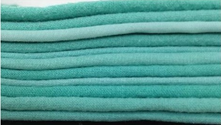
\includegraphics[width=\textwidth]{f901a.png}
		\caption{}\label{fig:f901a}
	\end{subfigure}
	\begin{subfigure}[b]{0.4\textwidth}
		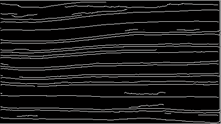
\includegraphics[width=\textwidth]{f901b.png}
		\caption{}\label{fig:f901b}
	\end{subfigure}
	\caption{(a) An original image (b) Edge detection}
	\label{fig:f901}
\end{figure}

Starting from an original input image is shown in Figure \ref{fig:f901a}. The edge detection is applied and the result image is shown in Figure \ref{fig:f901b}. In order to get feature of area and intensity the image is rotated 90 degree clockwise and the straight lines are drawn. The areas composed of the overlay straight lines and the edge produced edge detection can be obtained. The center of each area are found and marked with “o”. This is shown in Figure \ref{fig:f902}.
\begin{figure}[t]
	\centering
	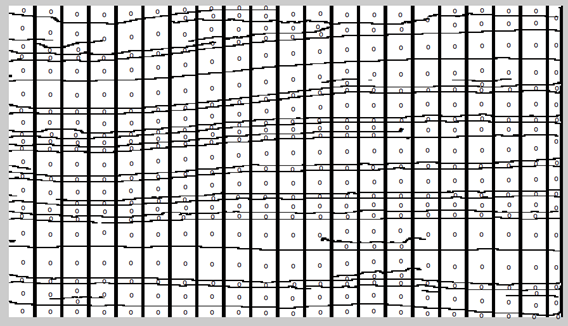
\includegraphics[scale=1]{f902.png}
	\caption{Area for calculating image features}
	\label{fig:f902}
\end{figure}

Figure \ref{fig:f903} plots the features obtained from each area. The horizontal axis represents the size of the area while the vertical axis represented the average intensity of each area. It is found that small size areas tens to be that area of cloth. However, the intensity of shadow and cloth area is not very well distinguishable.
\begin{figure}[t]
	\centering
	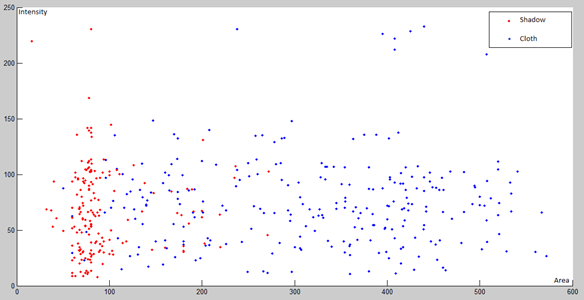
\includegraphics[scale=1]{f903.png}
	\caption{Features extraction of an input image}
	\label{fig:f903}
\end{figure} 

Thus, the result suggests that the classification using these two features and K-mean techniques cannot accomplish the classification task. This is because the features of shadow and sheets of cloth are not explicitly distinguishable. This means that the chosen features may be not proper for the task and the better features should be applied. By applying the good features, it should separate the data into different groups more clearly.

In summary, the feature of area intensity is not proper to use for classification in this project.
\section{Future work}
Nowadays, application counting sheets of cloth calculates number sheets of cloth with accuracy less than 80 percent because the application uses basic algorithm to calculate. So, first of all the algorithm should be improved for increasing accuracy. Addition, finding better features can classify data such as different color space of input image.